\section{Fit exploration}
\label{app:fit_exploration}
The fits below support the choice of the coupled Lorentzian power law (Sec.~\ref{sec:power_law}) and of the $\eta$ dependence (Sec.~\ref{sec:eta_dependence}). All fits are for $P_L=-2$, $|\vect b|\ge3a$ and $6\le\eta\le10$.


\subsection{Exponential decay in $|\vect b|$}

Fig.~\ref{fig:exp_straight} is the straight-line test for an exponential decay $\tAmp_{2B}^{\text{Re}}\propto e^{-c|\vect b|}$ in $|\vect b|=\sqrt{b^2}$. We fit $Ae^{-c|\vect b|}e^{-f\eta}$ with the loss of Eq.~\eqref{eq:pysr_loss}, which gives $c=0.685$ and $\mathcal L=1.42$ for three parameters, and $\mathcal L=1.31$ when a constant offset is added. For comparison, the \texttt{PySR} models of Table~\ref{tab:pysr_pareto} have $\mathcal L=1.61$ at $C=13$, $1.38$ at $C=15$ (five parameters) and $1.26$ at $C=17$. Over $3\le|\vect b|/a\le8.2$ the exponential in $|\vect b|$ therefore describes the data about as well as the power-law models, with fewer parameters. The search library has no function of $|\vect b|$ alone, so the Pareto front does not test this form. The separable ansätze of Sec.~\ref{sec:power_law} apply it to all three amplitudes.

\begin{figure*}[!p]
\centering
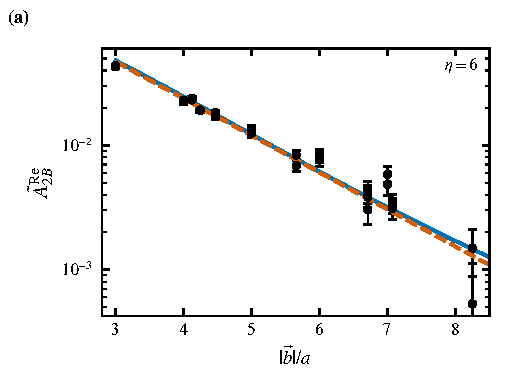
\includegraphics[width=\panelw]{figures/panels/pysr/exp_eta6.pdf}\hfill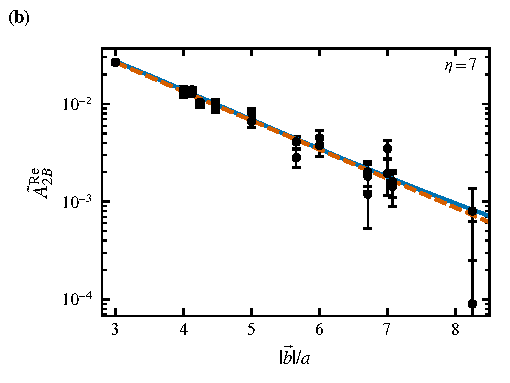
\includegraphics[width=\panelw]{figures/panels/pysr/exp_eta7.pdf}\par
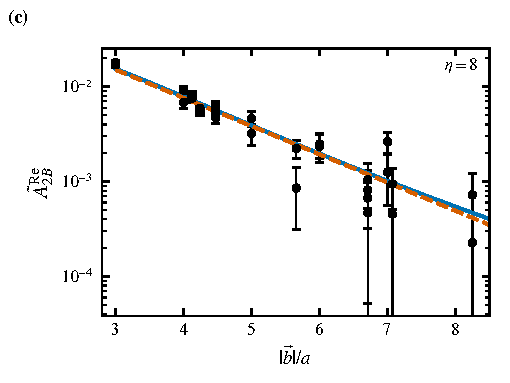
\includegraphics[width=\panelw]{figures/panels/pysr/exp_eta8.pdf}\hfill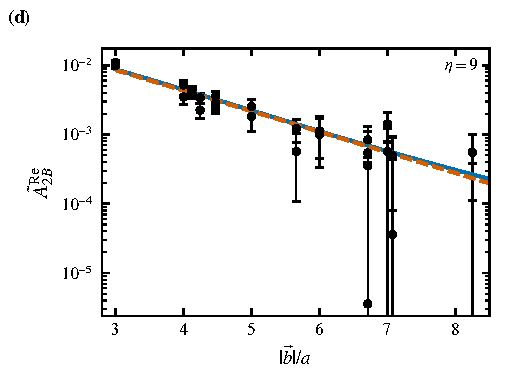
\includegraphics[width=\panelw]{figures/panels/pysr/exp_eta9.pdf}\par
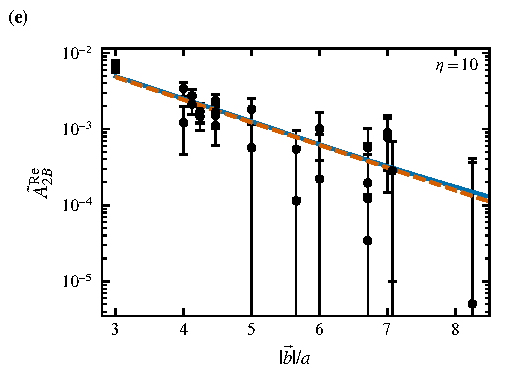
\includegraphics[width=\panelw]{figures/panels/pysr/exp_eta10.pdf}\hfill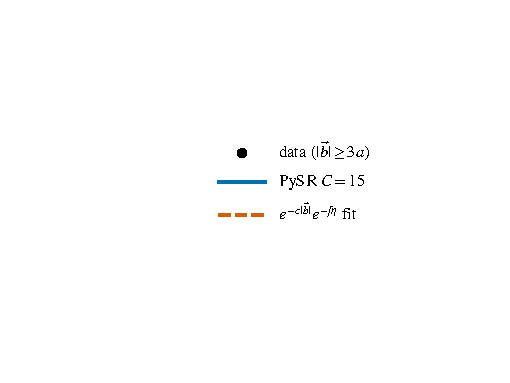
\includegraphics[width=\panelw]{figures/panels/pysr/exp_legend.pdf}
\caption{Panels (a)--(e): $\eta=6,7,8,9,10$. Straight-line test for an exponential decay in $|\vect b|=\sqrt{b^2}$ at $P_L=-2$. A profile $\tAmp_{2B}^{\text{Re}}\propto e^{-c|\vect b|}$ is a straight line on a logarithmic ordinate. The best fit (red dashed, $c=0.685$, $\mathcal L=1.42$) and the $C=15$ \texttt{PySR} model (blue, $\mathcal L=1.38$) both follow the data over $3\le|\vect b|/a\le8.2$.}
\label{fig:exp_straight}
\end{figure*}

\subsection{Gaussian and power-law fits with $\eta$-dependent widths}

Tables~\ref{tab:gauss_family_PL2} and~\ref{tab:powerlaw_family_PL2} list, for each model, the fit parameters and the correlated $\chi^2/\text{dof}$. The Gaussian ansätze reach $\chi^2/\text{dof}=1.56$ at best, against $1.10$ to $1.24$ for the power-law forms. The power-law forms with an $\eta$-dependent $c$ ($c(1-k_1/\eta)$, $c(1-k_1/\eta-k_2/\eta^2)$ and the wider forms) all give $\chi^2/\text{dof}\approx1.12$, so the data do not single out one $c(\eta)$, and the choice rests on the criteria of Sec.~\ref{sec:simultaneous_fit}.

Tables~\ref{tab:sep_EE_PL2}--\ref{tab:sep_EP_PL2} list separable ansätze, a longitudinal factor in $|b_LP_L|$ times a transverse factor in $b$, with the same $\eta$ dependences $c(\eta)$ of the longitudinal coefficient and a constant $d$: an exponential longitudinal and an exponential transverse factor, a power-law longitudinal and an exponential transverse factor, and an exponential longitudinal and a power-law transverse factor.

\begin{table*}
\caption{Fits of $\tAmp_{2B}^{\text{Re}}(b_L,b_T,\eta)$ at $P_L=-2$ ($|\vect b|\ge3a$, $6\le\eta\le10$) to $a\,e^{-f\eta}\exp[-c(\eta)(b_LP_L)^2-d(\eta)(b_L^2+b_T^2)]$. Each row $(i,j)$ uses $c(\eta)=c\,g_i(\eta)$ and $d(\eta)=d\,h_j(\eta)$ with $g_0=h_0=1$, $g_1=1-k_{c1}/\eta$, $g_2=1+k_{c1}/\eta-k_{c2}/\sqrt{\eta}$, $g_3=1-k_{c1}/\eta-k_{c2}/\eta^2$, and $h_1$, $h_2$, $h_3$ the same forms with $k_{d1}$, $k_{d2}$. Here $c$ multiplies $(b_LP_L)^2$, so it differs from the $c$ of the other tables by $P_L^2$. The $\chi^2/\mathrm{dof}$ is the correlated value with the full jackknife covariance matrix of the $\tAmp_{2B}^{\text{Re}}$ rows, from \texttt{lsqfit} (singular-value cut $10^{-12}$), given as the jackknife mean (error) over the 2903 jackknife columns (including the central value), as in the simultaneous fits, but without cross-amplitude correlations. The fits are unconstrained, and the number of degrees of freedom is the number of rows minus the number of parameters, counting all rows including the duplicated ($b_L\to-b_L$) rows. Rows marked with $^\dagger$ have shape parameters ($k_{\ldots}$, $\nu$) that are unconstrained (error $\ge$ value) or degenerate (value $>10^4$); only combinations of the parameters, not their individual values, are determined by the data.}
\label{tab:gauss_family_PL2}
\scriptsize
\begin{ruledtabular}
\begin{tabular}{l@{\hspace{3pt}}c@{\hspace{3pt}}c@{\hspace{3pt}}c@{\hspace{3pt}}c@{\hspace{3pt}}c@{\hspace{3pt}}c@{\hspace{3pt}}c@{\hspace{3pt}}c@{\hspace{3pt}}c}
$(i,j)$ & $a$ & $c$ & $k_{c1}$ & $k_{c2}$ & $d$ & $k_{d1}$ & $k_{d2}$ & $f$ & $\chi^2/\mathrm{dof}$ \\
\hline
$(0,0)$ & $2.09(14)$ & $-0.00169(68)$ &  &  & $0.0860(32)$ &  &  & $0.530(11)$ & $1.91(19)$ \\
$(0,1)$ & $0.918(94)$ & $-0.00116(66)$ &  &  & $0.173(11)$ & $2.88(17)$ &  & $0.382(18)$ & $1.57(17)$ \\
$(0,2)$ & $0.821(97)$ & $-0.00111(66)$ &  &  & $0.39(11)$ & $2.0(11)$ & $2.72(62)$ & $0.362(21)$ & $1.56(17)$ \\
$(0,3)$ & $0.837(98)$ & $-0.00111(66)$ &  &  & $0.231(37)$ & $5.2(10)$ & $-9.1(41)$ & $0.365(20)$ & $1.57(17)$ \\
$(1,0)$ & $1.52(12)$ & $0.0170(33)$ & $5.99(26)$ &  & $0.0840(31)$ &  &  & $0.474(13)$ & $1.74(18)$ \\
$(1,1)$$^\dagger$ & $0.934(97)$ & $0.0015(42)$ & $10(13)$ &  & $0.166(15)$ & $2.77(24)$ &  & $0.385(18)$ & $1.58(17)$ \\
$(1,2)$$^\dagger$ & $0.83(10)$ & $-0.0004(45)$ & $-10(336)$ &  & $0.39(12)$ & $2.0(12)$ & $2.71(64)$ & $0.363(22)$ & $1.57(17)$ \\
$(1,3)$$^\dagger$ & $0.85(10)$ & $-0.0001(32)$ & $0.0(15)\times10^{5}$ &  & $0.226(40)$ & $5.1(11)$ & $-9.0(43)$ & $0.367(21)$ & $1.58(17)$ \\
$(2,0)$$^\dagger$ & $1.51(12)$ & $0.044(42)$ & $1.6(45)$ & $3.1(18)$ & $0.0839(31)$ &  &  & $0.473(13)$ & $1.75(18)$ \\
$(2,1)$ & $0.875(94)$ & $0.088(40)$ & $6.31(58)$ & $5.05(25)$ & $0.173(16)$ & $2.90(23)$ &  & $0.373(19)$ & $1.57(17)$ \\
$(2,2)$$^\dagger$ & $0.86(11)$ & $0.072(60)$ & $6.33(71)$ & $5.07(31)$ & $0.23(18)$ & $-0.7(50)$ & $1.2(27)$ & $0.369(23)$ & $1.57(17)$ \\
$(2,3)$$^\dagger$ & $0.88(11)$ & $0.093(59)$ & $6.30(55)$ & $5.05(24)$ & $0.167(56)$ & $2.6(30)$ & $1(12)$ & $0.375(22)$ & $1.57(17)$ \\
$(3,0)$$^\dagger$ & $1.51(12)$ & $0.023(13)$ & $7.7(26)$ & $-11(16)$ & $0.0839(31)$ &  &  & $0.473(13)$ & $1.75(18)$ \\
$(3,1)$ & $0.881(94)$ & $0.023(12)$ & $13.0(14)$ & $-40.4(75)$ & $0.172(16)$ & $2.88(23)$ &  & $0.375(19)$ & $1.57(17)$ \\
$(3,2)$$^\dagger$ & $0.85(11)$ & $0.016(19)$ & $13.3(24)$ & $-41(12)$ & $0.27(18)$ & $0.3(37)$ & $1.7(21)$ & $0.368(23)$ & $1.58(17)$ \\
$(3,3)$$^\dagger$ & $0.88(11)$ & $0.022(18)$ & $13.0(15)$ & $-40.5(79)$ & $0.177(57)$ & $3.1(28)$ & $-1(11)$ & $0.374(22)$ & $1.58(17)$ \\
\end{tabular}
\end{ruledtabular}
\end{table*}

\begin{table*}
\caption{Fits of $\tAmp_{2B}^{\text{Re}}$ at $P_L=-2$ ($|\vect b|\ge3a$, $6\le\eta\le10$) to $a\,e^{-f\eta}\big/\{1+[d+c\,g(\eta)]b_L^2+d\,b_T^2\}^{j}$ for different $c(\eta)=c\,g(\eta)$. The $\chi^2/\mathrm{dof}$ is the correlated value, given as the jackknife mean (error).}
\label{tab:powerlaw_family_PL2}
\scriptsize
\begin{ruledtabular}
\begin{tabular}{l@{\hspace{3pt}}c@{\hspace{3pt}}c@{\hspace{3pt}}c@{\hspace{3pt}}c@{\hspace{3pt}}c@{\hspace{3pt}}c@{\hspace{3pt}}c@{\hspace{3pt}}c@{\hspace{3pt}}c@{\hspace{3pt}}c}
$c(\eta)$ & $a$ & $c$ & $d$ & $f$ & $k_1$ & $k_2$ & $k_3$ & $\nu$ & $j$ & $\chi^2/\mathrm{dof}$ \\
\hline
$c$ & $3.45(36)$ & $-0.0085(31)$ & $0.075(15)$ & $0.532(11)$ &  &  &  &  & $2.38(21)$ & $1.24(15)$ \\
$c(1-k_1/\eta)$ & $2.48(28)$ & $0.046(14)$ & $0.065(12)$ & $0.485(13)$ & $6.31(36)$ &  &  &  & $2.52(23)$ & $1.12(14)$ \\
$c(1-k_1/\eta-k_2/\eta^2)$ & $2.47(28)$ & $0.054(42)$ & $0.065(12)$ & $0.484(13)$ & $7.2(40)$ & $-6(25)$ &  &  & $2.52(23)$ & $1.12(14)$ \\
$c(1-k_1/\eta-k_2/\eta^2-k_3/\eta^3)$ & $2.48(28)$ & $0.85(44)$ & $0.067(13)$ & $0.482(13)$ & $20.37(52)$ & $-140.2(61)$ & $325(18)$ &  & $2.48(23)$ & $1.10(14)$ \\
$c(1-k_1\ln\eta/\eta)$ & $3.40(35)$ & $-2.86(77)\times10^{-8}$ & $0.076(15)$ & $0.528(11)$ & $-1.08(17)\times10^{6}$ &  &  &  & $2.37(21)$ & $1.23(15)$ \\
$c(1-k_1/\eta-k_2e^{-\nu\eta})$ & $2.49(28)$ & $-6.4(80)\times10^{-7}$ & $0.065(12)$ & $0.485(14)$ & $6.9(75)\times10^{5}$ & $-5.7(60)\times10^{5}$ &  & $0.261(80)$ & $2.52(23)$ & $1.13(14)$ \\
$c(1-k_1/\eta-k_2\ln\eta/\eta)$ & $2.53(28)$ & $-4.7(18)\times10^{-7}$ & $0.065(12)$ & $0.487(13)$ & $-1.13(35)\times10^{6}$ & $6.1(19)\times10^{5}$ &  &  & $2.51(23)$ & $1.13(14)$ \\
$c(1-k_1/\eta+k_2/\sqrt{\eta})$ & $2.47(28)$ & $0.10(13)$ & $0.065(12)$ & $0.484(13)$ & $-0.5(77)$ & $-2.7(31)$ &  &  & $2.52(23)$ & $1.12(14)$ \\
$c(1-k_1/\eta+k_2\ln\eta/\sqrt{\eta})$ & $2.46(28)$ & $0.17(26)$ & $0.065(12)$ & $0.483(13)$ & $1.9(24)$ & $-0.96(53)$ &  &  & $2.52(23)$ & $1.12(14)$ \\
$c\left(1+\dfrac{k_1\sqrt{\eta}}{1+k_2\eta}\right)$ & $2.47(28)$ & $0.093(69)$ & $0.065(12)$ & $0.484(13)$ & $0.0(21)\times10^{7}$ & $0.1(83)\times10^{6}$ &  &  & $2.52(23)$ & $1.12(14)$ \\
\end{tabular}
\end{ruledtabular}
\end{table*}

\begin{table*}
\caption{Fits of $\tAmp_{2B}^{\text{Re}}(b_L,b_T,\eta)$ at $P_L=-2$ ($|\vect b|\ge3a$, $6\le\eta\le10$) to $a\,e^{-f\eta}\exp[-c(\eta)|b_LP_L|]\,e^{-d|\vect b|}$ for different $c(\eta)$. Here $|\vect b|=\sqrt{b_L^2+b_T^2}$ and $b^2=b_L^2+b_T^2$. The $\chi^2/\mathrm{dof}$ is the correlated value, given as the jackknife mean (error).}
\label{tab:sep_EE_PL2}
\scriptsize
\begin{ruledtabular}
\begin{tabular}{l@{\hspace{3pt}}c@{\hspace{3pt}}c@{\hspace{3pt}}c@{\hspace{3pt}}c@{\hspace{3pt}}c@{\hspace{3pt}}c@{\hspace{3pt}}c@{\hspace{3pt}}c}
$c(\eta)$ & $a$ & $c$ & $k_1$ & $k_2$ & $k_3$ & $d$ & $f$ & $\chi^2/\mathrm{dof}$ \\
\hline
$c$ & $6.76(51)$ & $-0.0126(49)$ &  &  &  & $0.634(18)$ & $0.531(11)$ & $1.25(15)$ \\
$c(1-k_1/\eta)$ & $4.79(40)$ & $0.124(22)$ & $6.08(25)$ &  &  & $0.626(17)$ & $0.473(12)$ & $1.05(14)$ \\
$c(1-k_1/\eta-k_2/\eta^2)$ & $4.78(41)$ & $0.150(83)$ & $7.2(30)$ & $-7(18)$ &  & $0.625(17)$ & $0.472(13)$ & $1.06(14)$ \\
$c(1-k_1/\eta-k_2/\eta^2-k_3/\eta^3)$ & $4.76(40)$ & $1.27(59)$ & $19.73(83)$ & $-134.1(92)$ & $310(26)$ & $0.627(17)$ & $0.471(13)$ & $1.04(14)$ \\
$c(1-k_1/\sqrt{\eta})$ & $4.77(40)$ & $0.243(40)$ & $2.466(52)$ &  &  & $0.625(17)$ & $0.472(12)$ & $1.05(14)$ \\
\end{tabular}
\end{ruledtabular}
\end{table*}

\begin{table*}
\caption{Fits of $\tAmp_{2B}^{\text{Re}}(b_L,b_T,\eta)$ at $P_L=-2$ ($|\vect b|\ge3a$, $6\le\eta\le10$) to $a\,e^{-f\eta}\,[1+c(\eta)(b_LP_L)^2]^{-j}\,e^{-d|\vect b|}$ for different $c(\eta)$. Here $|\vect b|=\sqrt{b_L^2+b_T^2}$ and $b^2=b_L^2+b_T^2$. The $\chi^2/\mathrm{dof}$ is the correlated value, given as the jackknife mean (error).}
\label{tab:sep_PE_PL2}
\scriptsize
\begin{ruledtabular}
\begin{tabular}{l@{\hspace{3pt}}c@{\hspace{3pt}}c@{\hspace{3pt}}c@{\hspace{3pt}}c@{\hspace{3pt}}c@{\hspace{3pt}}c@{\hspace{3pt}}c@{\hspace{3pt}}c@{\hspace{3pt}}c}
$c(\eta)$ & $a$ & $c$ & $k_1$ & $k_2$ & $k_3$ & $d$ & $f$ & $j$ & $\chi^2/\mathrm{dof}$ \\
\hline
$c$ & $6.78(51)$ & $0.017(13)$ &  &  &  & $0.636(18)$ & $0.530(11)$ & $-0.16(10)$ & $1.25(15)$ \\
$c(1-k_1/\eta)$ & $4.89(42)$ & $0.20(55)$ & $5.95(11)$ &  &  & $0.615(13)$ & $0.480(13)$ & $0.14(26)$ & $1.09(14)$ \\
$c(1-k_1/\eta-k_2/\eta^2)$ & $4.84(42)$ & $2.8(96)$ & $11.5(16)$ & $-33.2(97)$ &  & $0.618(14)$ & $0.477(13)$ & $0.08(10)$ & $1.08(14)$ \\
$c(1-k_1/\eta-k_2/\eta^2-k_3/\eta^3)$ & $4.70(38)$ & $0.1(29)\times10^{5}$ & $20.96(33)$ & $-145.5(41)$ & $335(13)$ & $0.618(13)$ & $0.472(13)$ & $0.04(11)$ & $1.03(14)$ \\
$c(1-k_1/\sqrt{\eta})$ & $4.86(41)$ & $0.35(94)$ & $2.438(24)$ &  &  & $0.615(13)$ & $0.479(13)$ & $0.15(27)$ & $1.08(14)$ \\
\end{tabular}
\end{ruledtabular}
\end{table*}

\begin{table*}
\caption{Fits of $\tAmp_{2B}^{\text{Re}}(b_L,b_T,\eta)$ at $P_L=-2$ ($|\vect b|\ge3a$, $6\le\eta\le10$) to $a\,e^{-f\eta}\exp[-c(\eta)|b_LP_L|]\,(1+d\,b^2)^{-j}$ for different $c(\eta)$. Here $|\vect b|=\sqrt{b_L^2+b_T^2}$ and $b^2=b_L^2+b_T^2$. The $\chi^2/\mathrm{dof}$ is the correlated value, given as the jackknife mean (error).}
\label{tab:sep_EP_PL2}
\scriptsize
\begin{ruledtabular}
\begin{tabular}{l@{\hspace{3pt}}c@{\hspace{3pt}}c@{\hspace{3pt}}c@{\hspace{3pt}}c@{\hspace{3pt}}c@{\hspace{3pt}}c@{\hspace{3pt}}c@{\hspace{3pt}}c@{\hspace{3pt}}c}
$c(\eta)$ & $a$ & $c$ & $k_1$ & $k_2$ & $k_3$ & $d$ & $f$ & $j$ & $\chi^2/\mathrm{dof}$ \\
\hline
$c$ & $3.33(31)$ & $-0.0140(50)$ &  &  &  & $0.067(11)$ & $0.532(11)$ & $2.52(21)$ & $1.27(15)$ \\
$c(1-k_1/\eta)$ & $2.32(23)$ & $0.124(22)$ & $6.12(26)$ &  &  & $0.063(10)$ & $0.473(13)$ & $2.57(22)$ & $1.07(14)$ \\
$c(1-k_1/\eta-k_2/\eta^2)$ & $2.31(23)$ & $0.142(83)$ & $7.0(32)$ & $-5(20)$ &  & $0.062(10)$ & $0.473(13)$ & $2.57(22)$ & $1.08(14)$ \\
$c(1-k_1/\eta-k_2/\eta^2-k_3/\eta^3)$ & $2.31(23)$ & $1.29(59)$ & $19.82(80)$ & $-135.0(89)$ & $313(25)$ & $0.063(10)$ & $0.472(13)$ & $2.55(22)$ & $1.06(14)$ \\
$c(1-k_1/\sqrt{\eta})$ & $2.31(23)$ & $0.243(41)$ & $2.475(54)$ &  &  & $0.062(10)$ & $0.473(13)$ & $2.57(22)$ & $1.07(14)$ \\
\end{tabular}
\end{ruledtabular}
\end{table*}

